\documentclass[12pt,twoside]{article}

% Things that are not loaded by the package, though these might be
% generally useful.
\usepackage{natbib}
\usepackage{graphicx}
\setcounter{secnumdepth}{0}

% Load the package first - should sort everything out...
\usepackage{suppmat}

% ...and then we add some metadata
\titleprefix{Supporting information}
\runninghead{How much of the world is woody?}
\title{How much of the world is woody?}
\author{Richard G. FitzJohn$^{\dag, 1, 2}$, Matthew W. Pennell$^{\dag,3,4}$, Amy E. Zanne$^{5,6}$,\\ Peter F. Stevens$^{7,8}$, David C. Tank$^{3}$, and William K. Cornwell$^{9, 10}$}
\address{
\dag& These authors contributed equally\\
1& Biodiversity Research Centre \& Department of Zoology,
University of British Columbia\\
2& Department of Biological Sciences, Macquarie University\\
3& Department of Biological Sciences \& Institute for Bioinformatics
\& Evolutionary Studies, University of Idaho\\
4& National Evolutionary Synthesis Center\\
5& Department of Biological Sciences, George Washington University\\
6& Center for Conservation \& Sustainable Development, Missouri Botanical Garden\\
7& Department of Biology, University of Missouri\\
8& Missouri Botanical Garden\\
9& Department of Systems Ecology, VU University\\
10& Evolution \& Ecology Research Centre, School of Biological, Earth \& Environmental Sciences, University of New South Wales\\
}
\emailaddress{\email{rich.fitzjohn@gmail.com},\, \email{mwpennell@gmail.com}}
\date{}

\begin{document}

\maketitle

\section{Appendix S1: Survey details}

The survey we created is included as a Supplementary figure to
this paper (see \ref{fig:survey-text} and \ref{fig:survey-text-port}).
We distributed the survey to the 
community via several electronic
mailing lists with wide circulation among biologists: \emph{EvolDir},
\emph{ECOLOG}, \emph{\mbox{r-sig-phylo}}, \emph{Taxacom},
\emph{Herbaria}, as well as local lists. We also posted links on the
social--networking platforms \textsc{google+}, \textsc{twitter} and
\textsc{facebook} to reach a broad audience.
%
In order to increase representation of survey responses from Latin
America, we translated the survey into Portuguese and distributed it
to Brazilian biology \textsc{facebook} groups and university mailing
lists.

To analyse the survey data, we used linear regression on
logit--transformed percent woodiness as \citep[see][]{wartonarcsine}
and treated the self--reported level of botanical familiarity and
education as factors.  We converted country of training to coarse
latitude using shapefiles
from the GBIF dataportal\footnote{\url{http://code.google.com/p/gbif-dataportal/wiki/ConfiguringGeoserver}},
and converted these into ``tropical'' and ``temperate'' using an
absolute latitude of 23$^\circ$~26$^\prime$.  All analyses were
conducted with R version 3.0.2 \citep{R}.

\renewcommand\thefigure{S.\arabic{figure}}
\renewcommand\thetable{S.\arabic{table}}
\clearpage
\listoffigures

\begin{figure}[p]
  \centering
  \includegraphics[width=\textwidth]{figs/fraction-by-family}
  \caption[Distribution of woodiness proportion among
  families]{Distribution of the percentage of woodiness among
    families.
    The distribution of the percentage of species that are woody within
    a family is strongly bimodal among families (panel A), though less
    strongly bimodal than among genera.
    % 
    The two different sampling approaches generate distributions that
    differ in their bimodality (panel B).  Using the weak prior
    approach generates a broad distribution with many polymorphic
    genera (blue line), while using the strong prior approach
    generates a strongly bimodal distribution (red line).}
  \label{fig:distribution-family}
\end{figure}

\begin{figure}[p]
  \centering
  \includegraphics[width=\textwidth]{figs/fraction-by-order}
  \caption[Distribution of the percentage of woodiness among
  orders]{Distribution of the percentage of woodiness among orders.
    The distribution of the percentage of species that are woody within
    an order is bimodal among orders (panel A), though
    less strongly bimodal than among both genera and families.
    % 
    The two different sampling approaches generate distributions that
    differ in their bimodality (panel B).  Using the weak prior
    approach generates a broad distribution with many polymorphic
    genera (blue line), while using the strong prior approach
    generates a strongly bimodal distribution (red line).}
  \label{fig:distribution-order}
\end{figure}

\begin{figure}[p]
  \centering
  \includegraphics[width=\textwidth]{figs/distribution-raw}
  \caption[Estimates of woodiness proportion using both
  approaches]{The posterior probability distribution for
    the proportion of the world's flora that is woody, using our two
    sampling approaches.  The red (left) distribution samples missing
    species using the strong prior approach (binomial distribution),
    while the blue distribution (right) samples missing species using
    the weak prior approach (hypergeometric distribution).}
  \label{fig:distribution-raw}
\end{figure}

\begin{figure}[p]
  \centering
  \includegraphics[width=\textwidth]{figs/fraction-on-phylogeny-supp}
  \caption[Distribution of the fraction of woodiness among orders of vascular
  plants]{%
    \textit{This is Fig. 2 using the alternative sampling approach.}
    %
    Distribution of the fraction of woodiness among orders of vascular
    plants.  Each tip represents an order, with the fraction of
    circumference proportional to the square root of the number of
    recognised species in that order (data from accepted names in
    \citet{ThePlantList}).  The bars around the perimeter indicate the
    percentage of woody (black) and herbaceous (white) species,
    estimated using the ``weak prior'' (hypergeometric) approach.
    Using the ``strong prior'' (binomial) approach generally leads to
    an estimated percentage that is further away from 50\% (see
    main text Figs. 1 and 2).
    Phylogeny from \citet{Zanne} (available on Dryad;
    doi:10.5061/dryad.63q27/3). Orders not placed by APG III
    \citep{APG3} are not displayed.}
  \label{fig:phylogeny-supp}
\end{figure}

\begin{figure}[p]
  \centering
  \includegraphics[width=\textwidth]{figs/distribution-raw-errors}
  \caption[The effect of different coding on estimates]{The effect of
    different coding on estimates of the fraction of species that are
    woody, under the strong prior approach (binomial; panel A) and
    weak prior approach (hypergeometric; panel B).  The dark
    distributions are the results from our main analysis
    (Fig. \ref{fig:distribution-raw}).  Distributions to the left
    (with lower estimates of woodiness) code all species with any
    record of herbaceousness or variability as herbaceous.  Similarly,
    distributions to the right (with higher estimates of woodiness)
    code all species with any record of woodiness or variability as
    woody.}
  \label{fig:distribution-raw-errors}
\end{figure}
    
      
\begin{figure}[p]
  \centering
  \includegraphics[width=\textwidth]{figs/survey-distribution}
  \caption[Distribution of survey responses]{Distribution of all
    responses to the survey question ``What percentage of the world's
    vascular plant species are woody?''.
    %
    The mean and 95\% confidence intervals for our estimates of the
    proportion of woody species from the empirical data are depicted
    by the horizontal shaded rectangles; the blue rectangle
    corresponds to the ``weak prior'' approach and the red rectangle
    corresponds to the ``strong prior'' approach (see Appendix for
    details).  
    % 
    Panel A includes all 292 responses.  In panel B, the 282
    responses that indicated country are shown separated into
    ``tropical'' (orange distribution) and ``temperate'' (teal).
    Estimates from tropical countries were slightly, but
    significantly, higher than those from temperate countries
    ($p=$0.02, $r^2$=0.02).
    % #rstats
    % nrow(d.survey)                   # 292
    % sum(!is.na(d.survey$Country))    # 282
    % summary(res.tro)
  }

  \label{fig:survey-distribution}
\end{figure}

\begin{figure}[p]
  \centering
  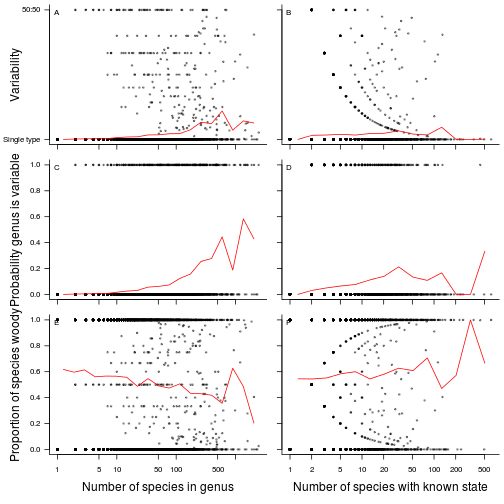
\includegraphics[width=.8\textwidth]{figs/variability}
  \caption[Relationship between genus size and proportion of
  woodiness]{The relationship between the size of a genus and its
    chance of being ``variable'' for woodiness.
%
We plotted the relationship between the level of variablitiy in the
dataset (from all of a single--type to equal numbers of woody and
herbaceous species) against the number of species in a genus (panel A)
and the number of species with known state (panel B). Larger genera
tend to be more variable although this pattern is not strong. We then
coded all genera as being either variable or all of a single--type and
examined the relationship between this binary characterization and the
number of species per genus (panel C) and the number for which we
have known states (panel D). Using the binary characterization, it is
clear that large genera have a higher probability of being variable,
even if few species actually vary (compare with panels A and
B). Though there is a great deal of scatter, larger genera also tend to be
more herbaceous than woody genera (panel E) but the genera for which
we have more data tend to be more woody (panel F). This shows that the
available data is generally biased towards woody species.  In all
panels, the red line is a moving average over 20 (left column) of 15 (right
column) equally spaced bins on this log axis.}
  \label{fig:variability}
\end{figure}

\begin{figure}[p]
  \centering
  \vspace{-20ex}
  \includegraphics[height=.93\textheight]{figs/Survey_supplemental}
  \caption{English--language version of the survey we distributed}
  \label{fig:survey-text}
\end{figure}

\begin{figure}[p]
  \centering
  \vspace{-20ex}
  \includegraphics[height=.93\textheight]{figs/Survey_supplemental_Portuguese}
  \caption{Portuguese--language version of the survey we distributed}
  \label{fig:survey-text-port}
\end{figure}

\clearpage

\bibliographystyle{jecol}
\bibliography{wood.bib}


\end{document}

%%% Local Variables:
%%% mode: latex
%%% TeX-master: t
%%% TeX-PDF-mode: t
%%% End:
